\section{Arquitectura}

En esta secci\'on presentaremos y analizaremos la arquitectura pensada para resolver el trabajo, as\'i como las t\'acticas utilizadas para asegurar los atributos de calidad que se mencionaron anteriormente.

\subsection{Comunicaci\'on con Drones}

Para el monitoreo de las plantaciones se utilizar\'an drones que tomar\'an fotograf\'ias y luego ser\'an analizadas para recaudar la informaci\'on necesaria.  Para esto, contamos con un componente dedicado a la comunicaci\'on con las interfaces de manejo de drones que nos provee el Ministerio y la empresa privada. Se utilizar\'a por default el sistema de drones estatales, en caso de no responder a los pedidos, se pasara a utilizar el sistema privado.

A medida que se reciben las im\'agenes, se pasan utilizando una cola al geolocalizador que se encarga de identificar las plantaciones: analizando las im\'agenes y usando la informaci\'on del repositorio de geolocalizaciones. Este componente se encarga tambi\'en de descartar las im\'agenes err\'oneas que no permiten un an\'alisis.

El repositorio contiene informaci\'on ingresada por los usuarios sobre la localizaci\'on de las plantaciones, as\'i como su estado. Esta informaci\'on se utiliza para comparar con el an\'alisis que haga el geolocalizador y poder verificar de qu\'e plantaci\'on se trata.

Una vez tageada la imagen se env\'ia a los analizadores que trabajan en paralelo para reconocer la T\textdegree, el estado del suelo y la salinidad del agua. Luego de esto se procede a mergear los resultados y guardarlos en el repo de informaci\'on.

Por \'ultimo, el manager de monitoreo de im\'agenes se encarga de ir agregando los pedidos que deben realizarse para que luego se vayan realizando. Para esto est\'a el repo de pedidos d\'onde el componente que pide las im\'agenes se conecta de manera blackboard y luego realiza la solicitud usando el comunicador con los drones.

\begin{figure}[h!]
  \centering
  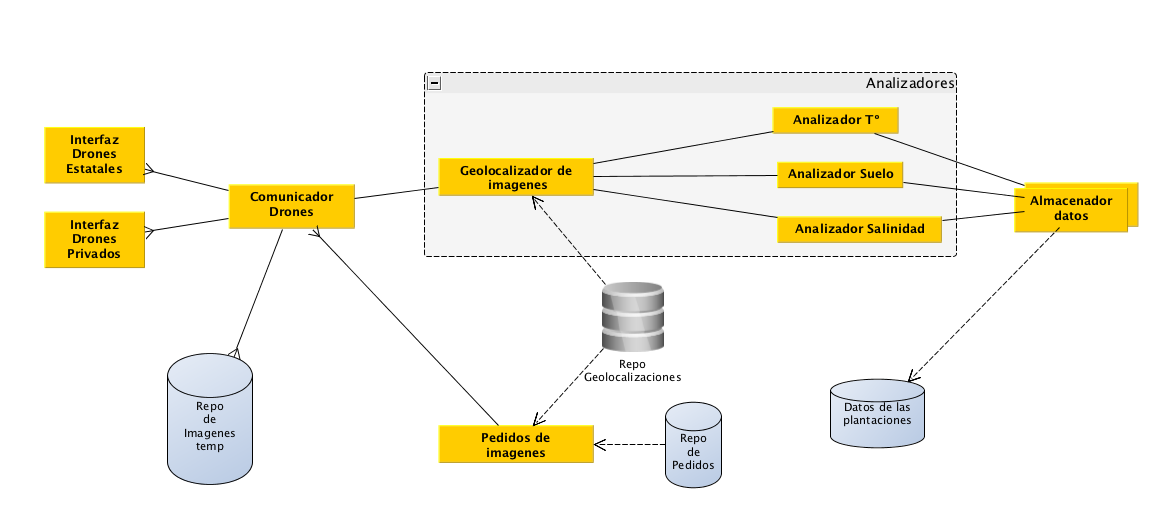
\includegraphics[width=1\textwidth]{./images/arq_drones.png}
  \caption{Arquitectura de comunicaci\'on con drones y procesamiento de im\'agenes}
  \label{fig:clases4}
\end{figure}

\subsection{Comunicaci\'on con estaciones meteorol\'ogicas}

El mecanismo es bastante similar a la comunicaci\'on con drones. El comunicador establece el pedido con la estaci\'on meteorol\'ogica y luego env\'ia el paquete usando una cola al analizador, quien luego se lo env\'ia al almacenados de datos que lo agrega al repo.

\begin{figure}[h!]
  \centering
  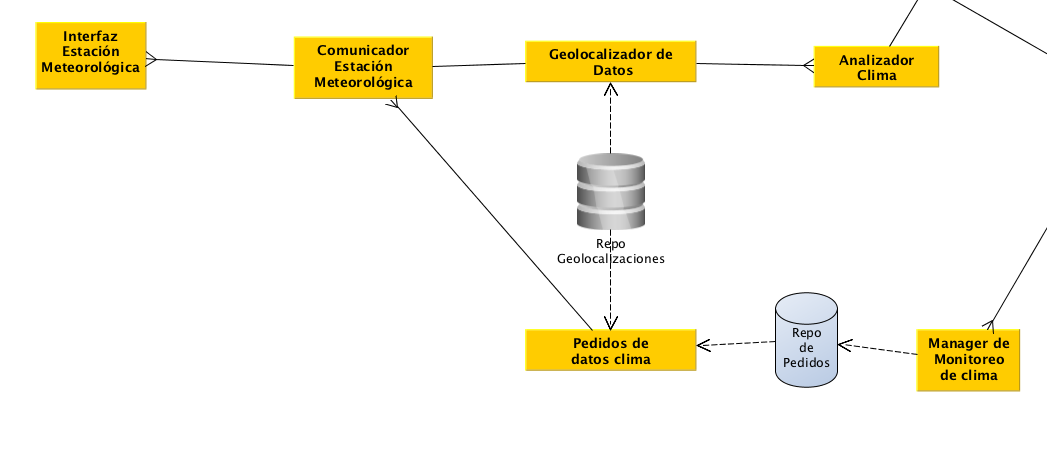
\includegraphics[width=1\textwidth]{./images/arq_clima.png}
  \caption{Arquitectura de comunicaci\'on con estaciones meteorol\'ogicas y procesamiento de datos}
  \label{fig:clases4}
\end{figure}


\subsection{Comunicaci\'on con Interfaz de usuarios}

Utilizando la interfaz de usuario, se permite agregar datos sobre las plantaciones de manera manual. Tambi\'en se realiza la configuraci\'on de monitoreo de clima y de im\'agenes (frecuencia, horarios, etc).

\begin{figure}[h!]
  \centering
  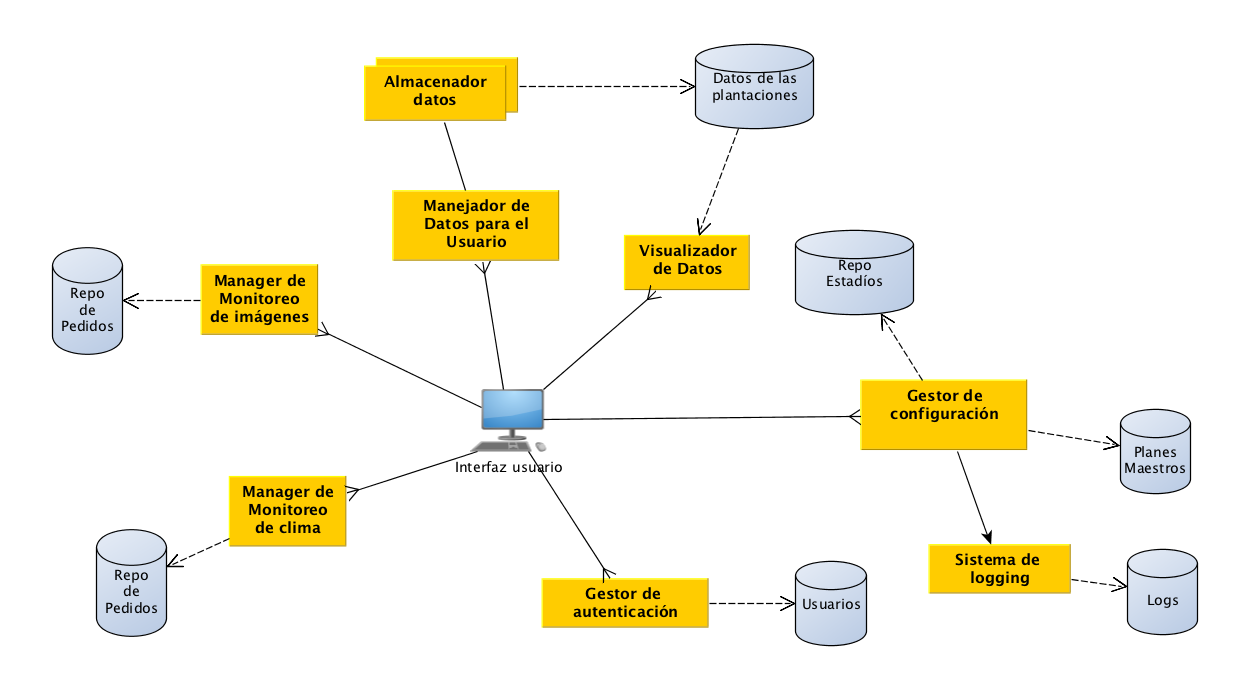
\includegraphics[width=0.4\textwidth]{./images/arq_interfazusuario.png}
  \caption{Arquitectura de comunicaci\'on con la interfaz de usuario}
  \label{fig:clases4}
\end{figure}

\subsection{Planificaci\'on}

Con la informaci\'on almacenada en los repositorios, el planificador arma los eventos que deben realizarse para continuar con el plan de trabajo deseado.

\begin{figure}[h!]
  \centering
  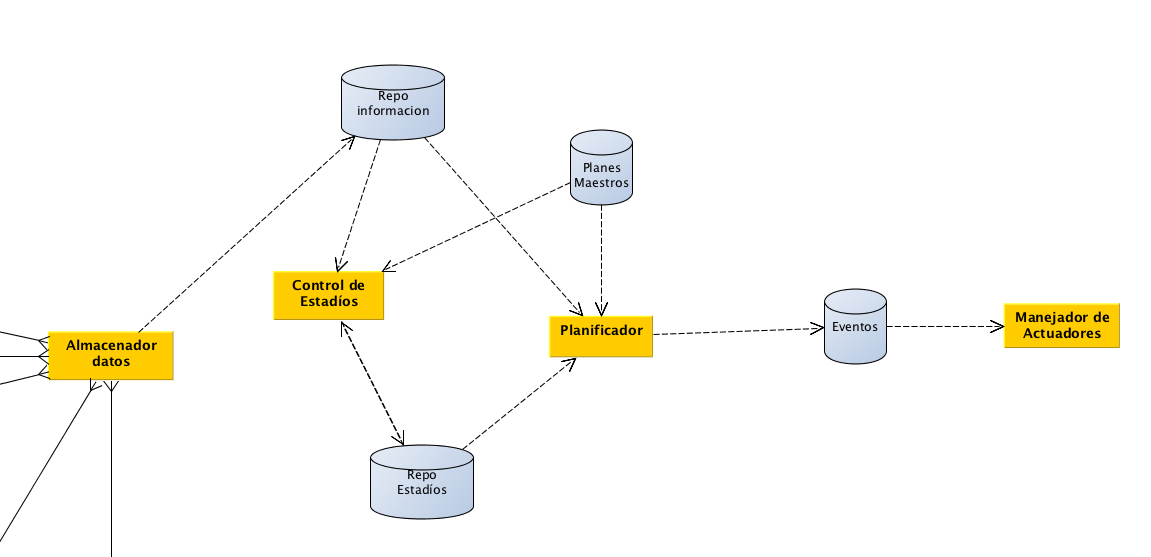
\includegraphics[width=1\textwidth]{./images/arq_plan.png}
  \caption{Arquitectura de planificaci\'on de eventos}
  \label{fig:clases4}
\end{figure}
